\section{Results and Discussion}
\label{sec:results}

\subsection{Evaluation of Label Efficiency}
\label{subsec:res_label_efficiency}

\begin{figure}[t]
    \centering
    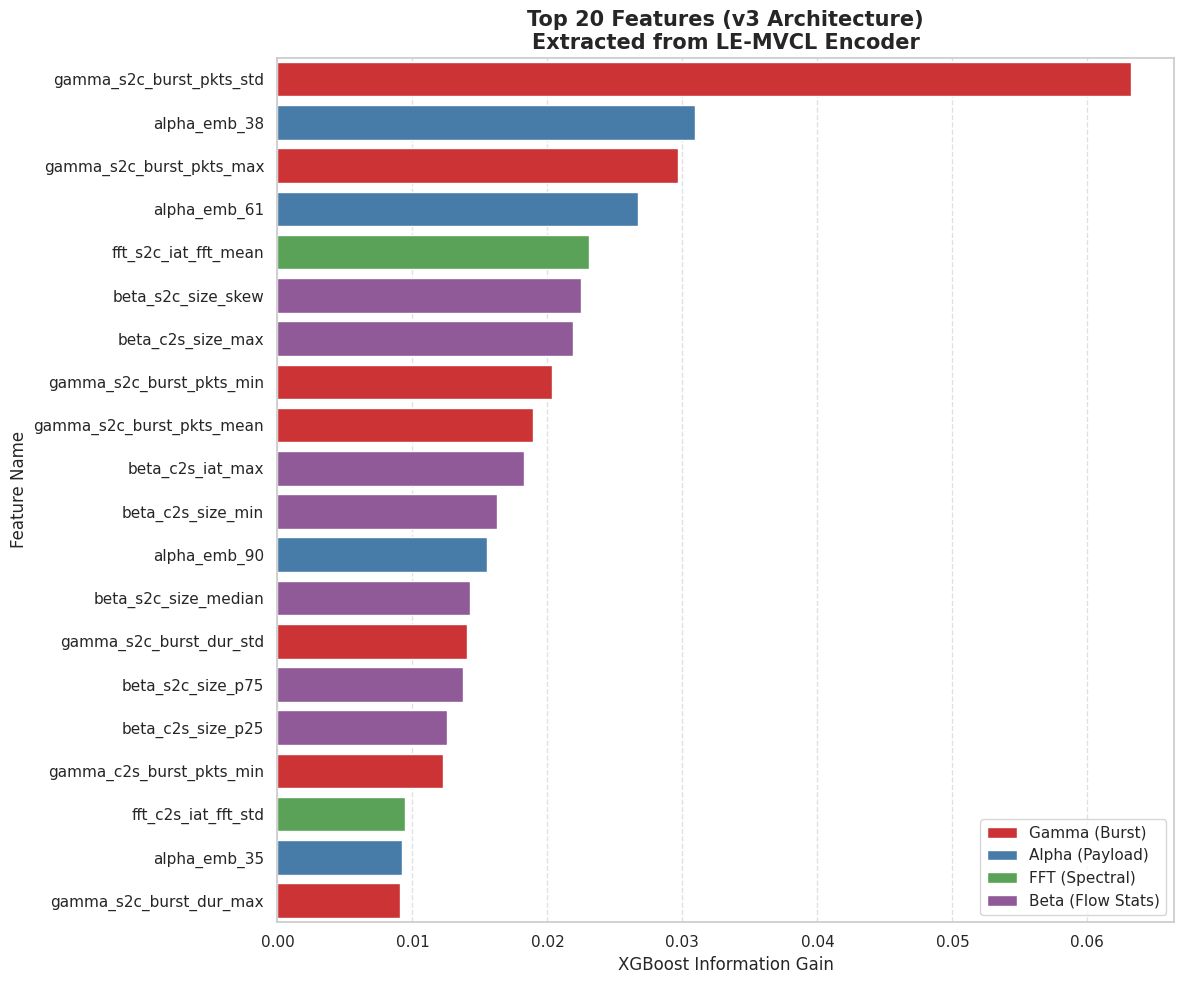
\includegraphics[width=\columnwidth]{img/rank.png}
    \caption{Global Feature Importance. The top 20 features reveal a hybrid dependency, where Gamma (Burst) features provide the highest information gain, supported by learned Alpha (Payload) embeddings.}
    \label{fig:rank}
\end{figure}

\begin{figure}[t]
    \centering
    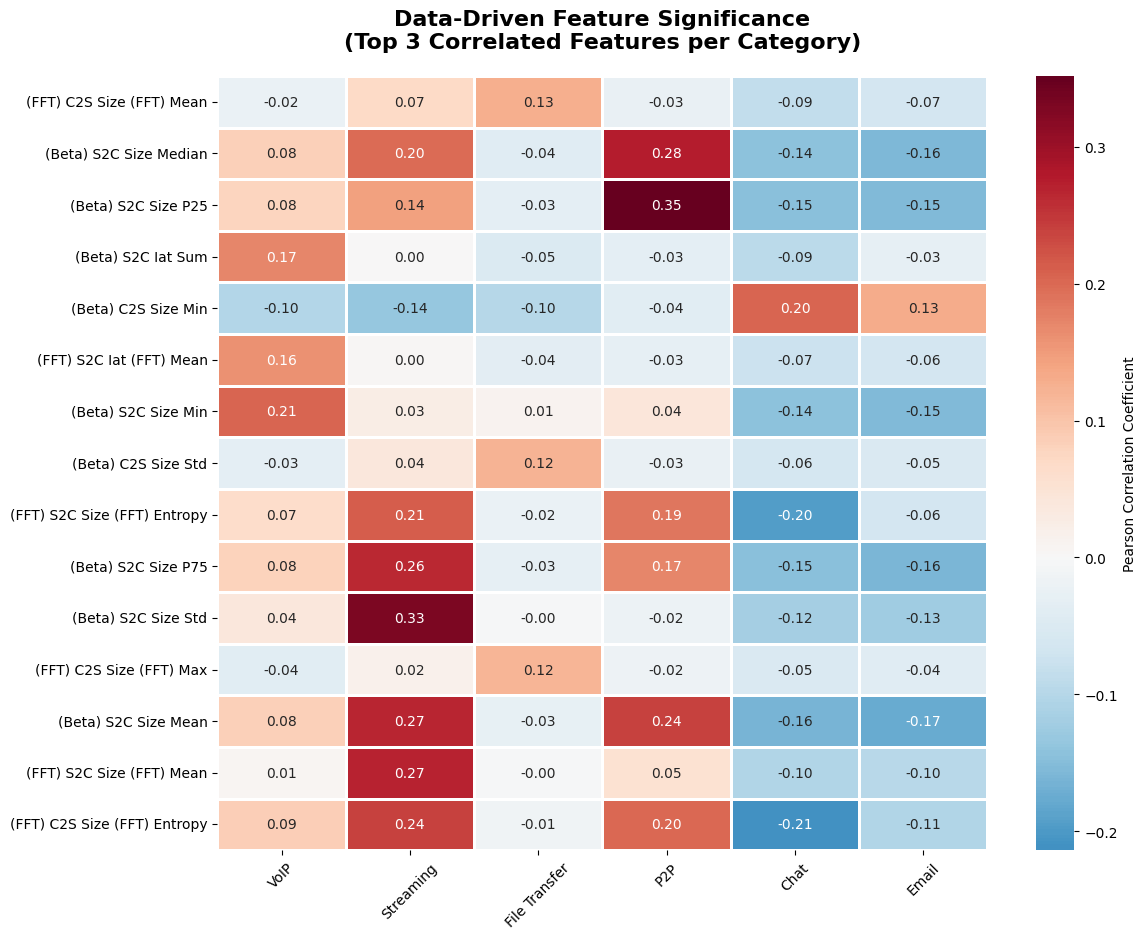
\includegraphics[width=\columnwidth]{img/featurecorrelationtop3.png}
    \caption{Linear Correlation Matrix. Beta features exhibit strong linear relationships, whereas the high-importance Gamma features are absent, highlighting the non-linear nature of burst dynamics.}
    \label{fig:correlation}
\end{figure}

\begin{figure*}[t]
    \centering
    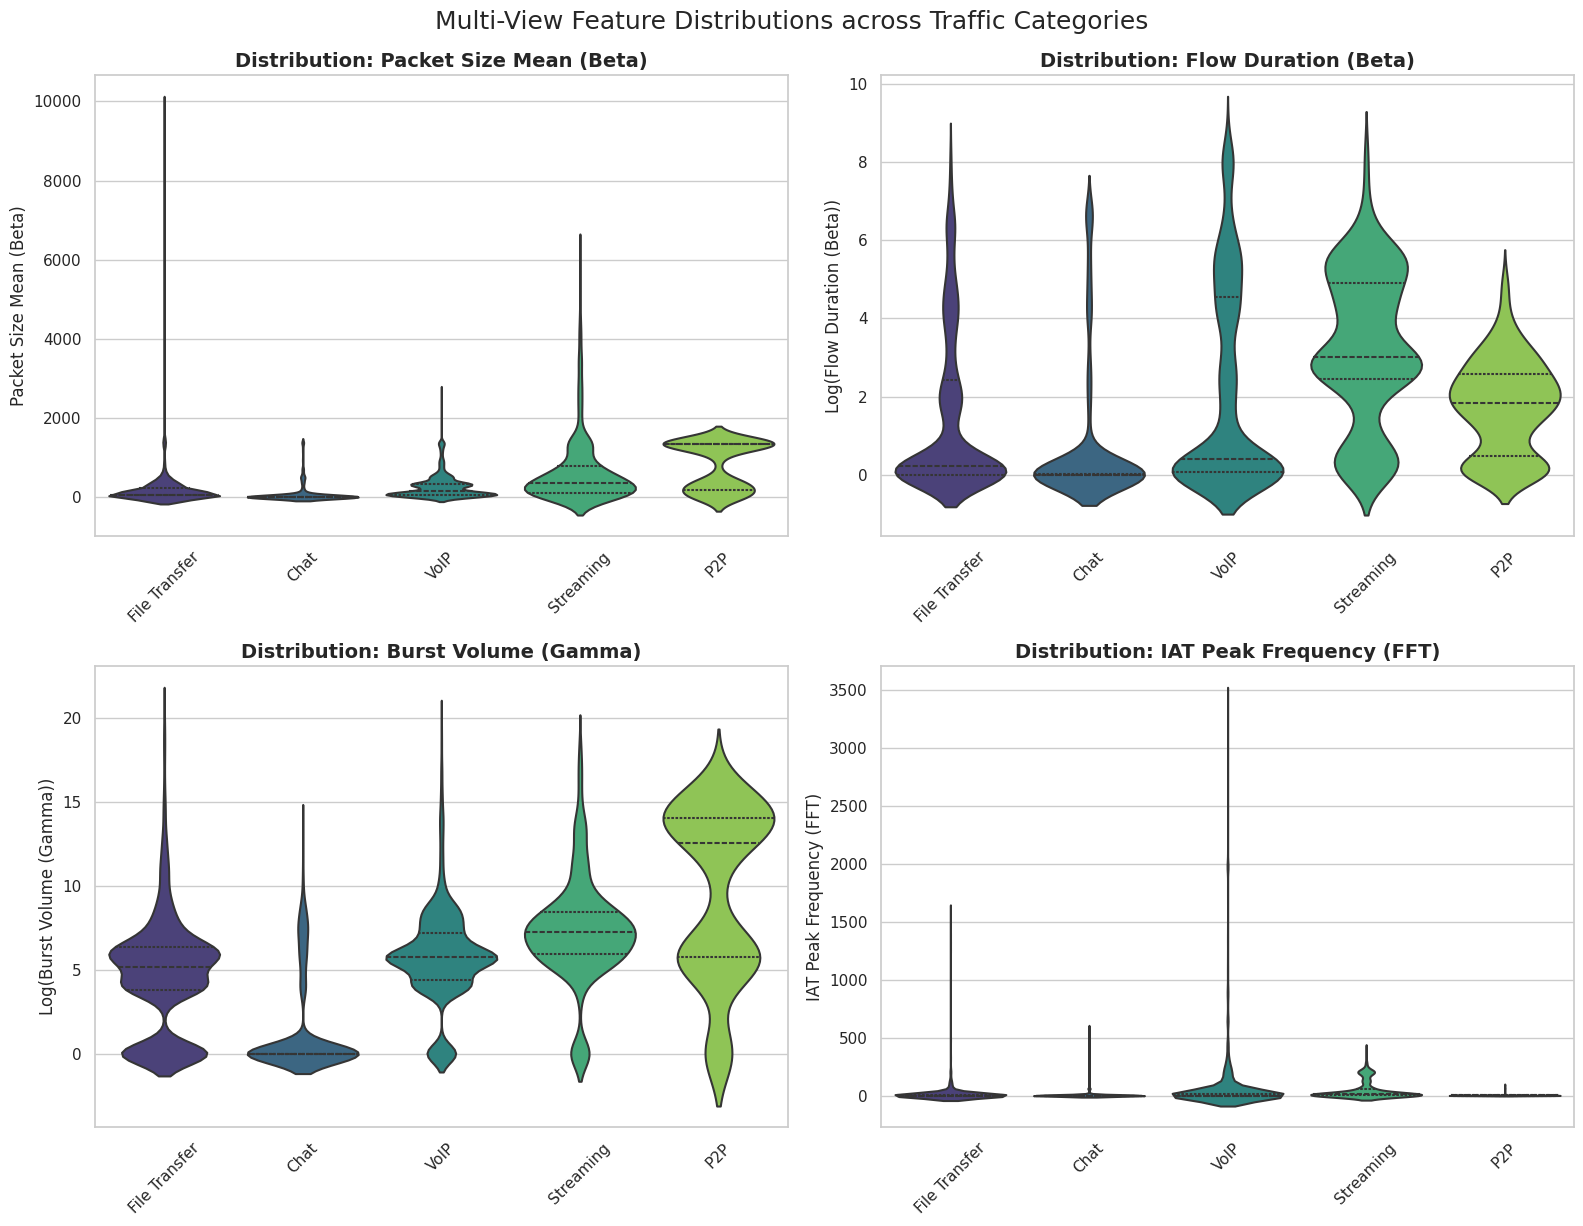
\includegraphics[width=\textwidth]{img/violin.png}
    \caption{Multi-View Feature Distributions. Different views resolve different ambiguities: Beta isolates bulk P2P transfer, Gamma separates high-volume Streaming, and FFT uniquely identifies the periodic signature of VoIP.}
    \label{fig:violin}
\end{figure*}

\begin{figure}[t]
    \centering
    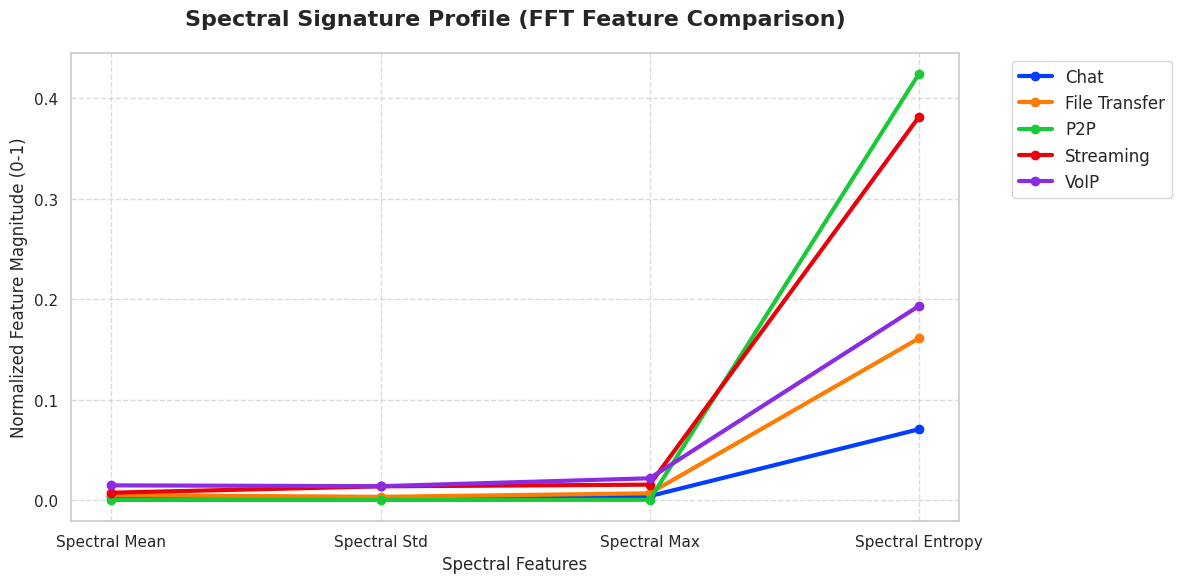
\includegraphics[width=\columnwidth]{img/spectral.png}
    \caption{Spectral Signature Profile. A parallel coordinates plot demonstrating the "Spectral Crossover": VoIP is characterized by high Periodicity (Max) and low Entropy, whereas P2P/Streaming exhibit the inverse.}
    \label{fig:spectral}
\end{figure}

\begin{figure}[t]
    \centering
    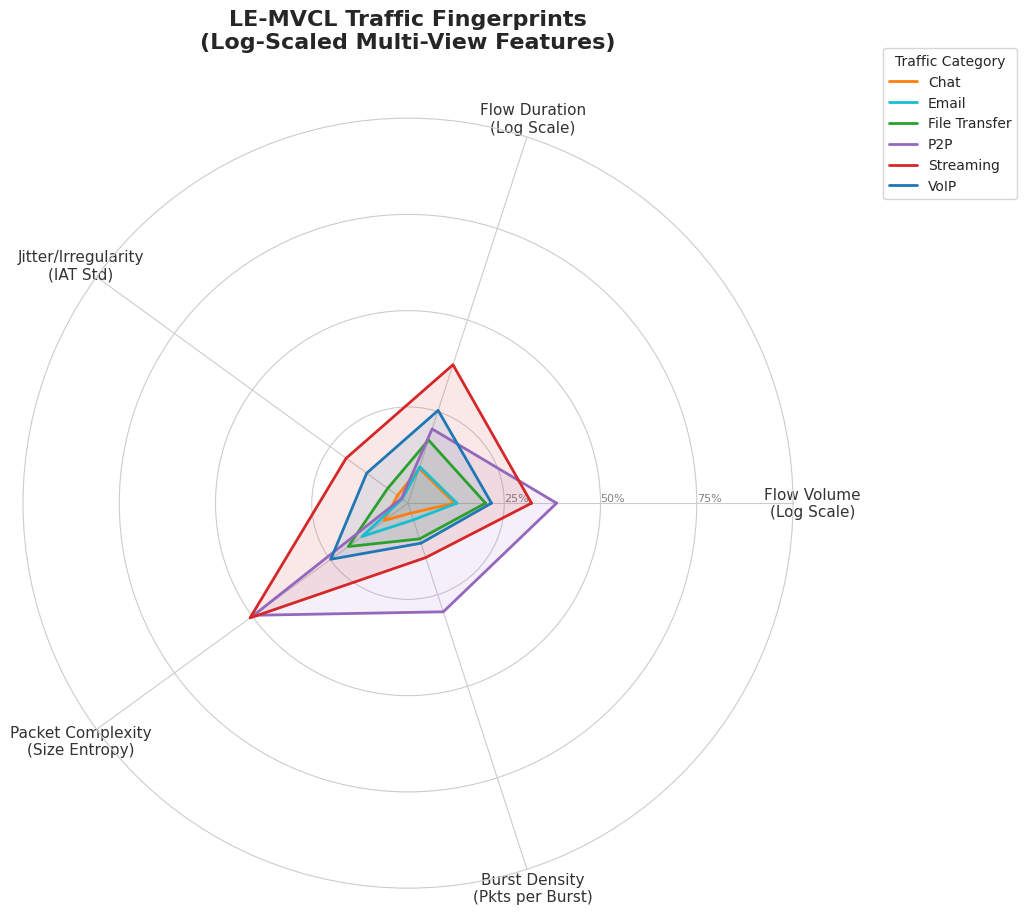
\includegraphics[width=\columnwidth]{img/spider.png}
    \caption{Holistic Traffic Fingerprints. Radar charts illustrate the unique multi-view geometry of each class, showing how LE-MVCL leverages orthogonal features to create separable signatures.}
    \label{fig:spider}
\end{figure}

\begin{figure*}[t]
    \centering
    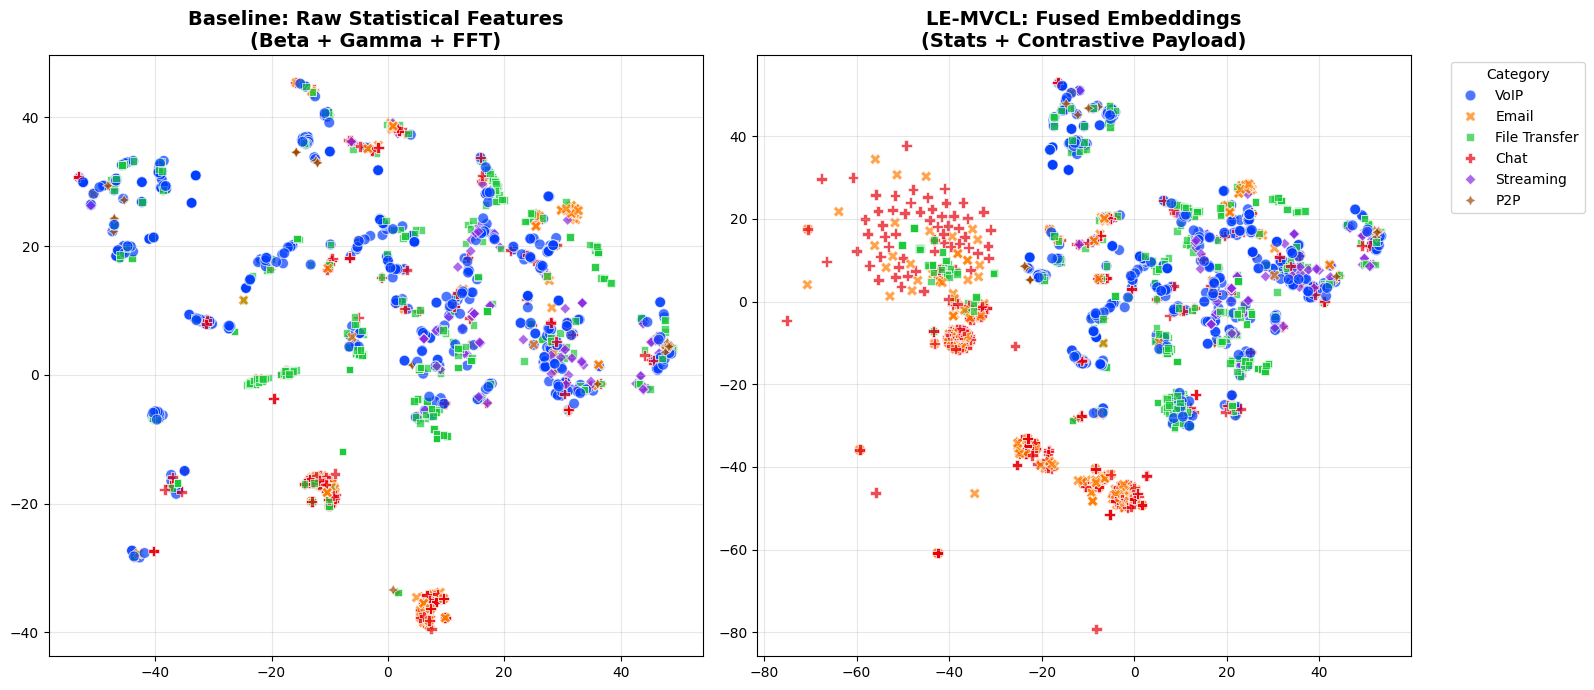
\includegraphics[width=\textwidth]{img/tsne.png}
    \caption{Manifold Projection (t-SNE). Left: The baseline using only raw statistical features shows high confusion between interactive classes (VoIP/Chat). Right: LE-MVCL's Hybrid Fusion creates distinct, compact clusters, proving that the semantic "Alpha" embeddings successfully disentangle classes that are statistically similar.}
    \label{fig:tsne}
\end{figure*}

The primary hypothesis driving this research is that asymmetric contrastive pre-training can effectively mitigate the dependency on large-scale labeled datasets in encrypted traffic analysis. To validate this, we conducted a rigorous comparative evaluation against state-of-the-art supervised baselines, measuring performance degradation as label availability was restricted to 5\%, 10\%, 20\%, and 30\% of the training corpus.

To ensure a fair comparison of \textit{label efficiency}, we reproduced two established architectures: the 1D-CNN proposed by Wang et al. \cite{wang2017end} and Deep Packet by Lotfollahi et al. \cite{lotfollahi2020deep}. It is important to note the distinction in data access: supervised baselines are trained \textit{exclusively} on the labeled subset (e.g., 5\%) as they lack mechanisms to process unlabeled data. In contrast, LE-MVCL utilizes the remaining unlabeled portion of the dataset during the pre-training phase. This setup mirrors the real-world operational constraint where unlabeled traffic is abundant (free), but ground-truth labels are scarce (expensive). Thus, the comparison measures the \textit{value of leveraging unlabeled data} rather than pure sample efficiency.

\subsubsection{Performance Trajectory of LE-MVCL}
We first analyze the performance of the proposed LE-MVCL framework across the three hierarchical tasks: Binary Detection (Encrypted Gatekeeper), Category Classification, and Fine-Grained Application Identification. As shown in Table \ref{tab:lemvcl_trajectory}, LE-MVCL demonstrates robust scalability.

In the Binary task, the model achieves a strong F1-score of 89.8\% with only 5\% of the data, rapidly converging to 94.9\% at 30\% availability. This confirms the effectiveness of the pre-trained encoder in distinguishing fundamental encrypted tunnel structures from background traffic. For the more challenging fine-grained Application task, LE-MVCL maintains an F1-score of 75.2\% under extreme scarcity, which improves significantly to 91.3\% as more labels become available. This trajectory indicates that while the "cold start" performance is competitive, the model is highly responsive to additional supervision, effectively refining its decision boundaries for complex services like BitTorrent and Skype.

\begin{table}[htbp]
\caption{Performance Trajectory of LE-MVCL (Macro F1-Score)}
\label{tab:lemvcl_trajectory}
\centering
\begin{tabular}{l c c c c}
\hline
\textbf{Task} & \textbf{5\%} & \textbf{10\%} & \textbf{20\%} & \textbf{30\%} \\
\hline
Binary Detection & 89.8\% & 92.2\% & 94.5\% & 94.9\% \\
VPN Category & 70.7\% & 78.7\% & 84.8\% & 87.1\% \\
VPN Application & 75.2\% & 84.6\% & 90.0\% & 91.3\% \\
\hline
\end{tabular}
\end{table}

\subsubsection{Comparative Analysis with Baselines}
To benchmark these results, we compared LE-MVCL against four baselines: a lightweight statistical model (Stats-Only), two supervised deep learning models (1D-CNN, Deep Packet), and a symmetric contrastive model (SimCLR). Table \ref{tab:baseline_comparison} summarizes the performance gap ($\Delta$) between each baseline and LE-MVCL at the critical 5\% and 30\% thresholds.

\begin{table*}[htbp]
\caption{Comprehensive Baseline Comparison (Macro F1-Score). \\ Models marked with ($^\dagger$) utilize unlabeled data for pre-training (Semi-Supervised), while others rely solely on the labeled subset (Supervised).}
\label{tab:baseline_comprehensive}
\centering
\resizebox{\textwidth}{!}{%
\begin{tabular}{l | c c c c | c c c c | c c c c}
\hline
\multirow{2}{*}{\textbf{Model}} & \multicolumn{4}{c|}{\textbf{Binary Detection}} & \multicolumn{4}{c|}{\textbf{VPN Category}} & \multicolumn{4}{c}{\textbf{VPN Application}} \\
 & \textbf{5\%} & \textbf{10\%} & \textbf{20\%} & \textbf{30\%} & \textbf{5\%} & \textbf{10\%} & \textbf{20\%} & \textbf{30\%} & \textbf{5\%} & \textbf{10\%} & \textbf{20\%} & \textbf{30\%} \\
\hline
Stats-Only (XGB) & \textbf{91.0} & 92.0 & 93.0 & 94.0 & 72.0 & \textbf{79.0} & \textbf{87.0} & \textbf{89.0} & 74.0 & 83.0 & 87.0 & 88.0 \\
1D-CNN \cite{wang2017end} & 83.5 & 86.0 & 89.3 & 89.4 & 66.3 & 74.2 & 79.3 & 83.6 & 76.1 & 80.3 & 86.8 & 86.5 \\
Deep Packet \cite{lotfollahi2020deep} & 80.6 & 85.0 & 88.6 & 89.2 & 67.8 & 75.8 & 78.6 & 83.2 & 75.4 & 83.4 & 86.5 & 87.4 \\
Deep Fusion \cite{zeng2019deep} & 85.0 & 88.0 & 90.0 & 91.0 & \textbf{75.0} & 78.0 & 83.0 & 84.0 & \textbf{84.0} & 85.0 & 89.0 & 91.0 \\
\hline
SimCLR (Symmetric) $^\dagger$ & 88.4 & 91.9 & 93.1 & 93.5 & 65.2 & 78.1 & 82.2 & 85.8 & 70.4 & \textbf{85.5} & 88.2 & 89.5 \\
\textbf{LE-MVCL (Ours)} $^\dagger$ & 89.8 & \textbf{92.2} & \textbf{94.5} & \textbf{94.9} & 70.7 & 78.7 & 84.8 & 87.1 & 75.2 & 84.6 & \textbf{90.0} & \textbf{91.3} \\
\hline
\end{tabular}%
}
\end{table*}

Superiority in Binary Detection:
LE-MVCL consistently outperforms the deep learning baselines in the binary task. At 5\% labels, it exceeds the Supervised 1D-CNN by 6.3\% and Deep Packet by 9.2\%. While the Stats-Only model shows a slight initial advantage (+1.2\%), LE-MVCL overtakes it at 30\% (+0.9\%), proving that the learned payload representations provide scalability that pure statistics lack.

Scalability in Fine-Grained Tasks:
In the application identification task, LE-MVCL demonstrates superior long-term performance. At 30\% label density, it achieves the highest F1-score of 91.3\%, surpassing Stats-Only (88.0\%) and SimCLR (89.5\%). Although the Deep Fusion baseline shows strong initial performance in Application identification at 5\%, LE-MVCL closes the gap at 30\% (91.3\% vs 91.0\%), while consistently outperforming it in the Binary domain (89.8\% vs 85.0\% at 5\% labels), highlighting the robustness of our Direct Fusion strategy.

\subsection{Hierarchical Classification Performance}
\label{subsec:res_hierarchical}

We further evaluate the system's reliability by examining the class-wise performance of the "VPN Specialist" module. Table \ref{tab:hierarchical_breakdown} details the F1-scores for the top 6 VPN applications.

\begin{table}[htbp]
\caption{Stage 2: VPN Specialist Performance (Top-6 Apps, Macro F1)}
\label{tab:hierarchical_breakdown}
\centering
\scriptsize
\setlength{\tabcolsep}{3pt}
\resizebox{\columnwidth}{!}{%
\begin{tabular}{p{0.55\columnwidth} c c}
\hline
\textbf{Application} & \textbf{5\% Labels (F1)} & \textbf{30\% Labels (F1)} \\
\hline
VPN\_BitTorrent & 0.84 & 0.97 \\
VPN\_Skype & 0.86 & 0.97 \\
VPN\_Email & 0.79 & 0.92 \\
VPN\_YouTube & 0.76 & 0.95 \\
VPN\_Hangout & 0.73 & 0.87 \\
VPN\_Facebook & 0.54 & 0.80 \\
\hline
\textbf{Macro Average} & \textbf{0.75} & \textbf{0.91} \\
\hline
\end{tabular}%
}
\end{table}

The results show exceptional recovery for minority and complex classes. \textit{VPN\_BitTorrent}, often difficult due to its P2P nature, reaches a near-perfect 0.97 F1 at 30\%. \textit{VPN\_Skype} similarly hits 0.97. The most challenging class, \textit{VPN\_Facebook} (likely due to its multimodal mix of video and chat), sees a massive improvement from 0.54 to 0.80 as supervision increases, confirming that the model successfully disentangles it from similar Google services (YouTube/Hangout) when given sufficient examples.

\subsubsection{Cross-Domain Robustness (VNAT)}
Finally, to validate generalization, we tested the Binary Gatekeeper on the VNAT dataset (Table \ref{tab:binary_vnat}) using a Transfer Learning approach. The model achieved a sensitive Macro F1 of 98.33\% with only 5\% labeled data, demonstrating immediate adaptability. Performance remained stable across all label densities (98.24\% at 10\%, 97.99\% at 20\%, and 97.70\% at 30\%), proving that the learned features are robust and transferable across different network environments without extensive retraining.

\begin{table}[htbp]
\caption{Stage 1: Binary Gatekeeper Performance (VNAT Dataset)}
\label{tab:binary_vnat}
\centering
\scriptsize
\setlength{\tabcolsep}{3pt}
\resizebox{\columnwidth}{!}{%
\begin{tabular}{p{0.38\columnwidth} c c c c}
\hline
\textbf{Metric} & \textbf{5\% Labels} & \textbf{10\% Labels} & \textbf{20\% Labels} & \textbf{30\% Labels} \\
\hline
\textbf{Macro F1} & 98.33\% & 98.24\% & 97.99\% & 97.70\% \\
\hline
\end{tabular}%
}
\end{table}

\subsection{Multi-View Feature Analysis}
\label{subsec:feature_analysis}

To validate the LE-MVCL hypothesis—that encrypted traffic requires complementary feature views—we conducted a comprehensive analysis of feature importance, correlation, and spectral behavior.

\subsubsection{Global Feature Importance}
We first analyzed the global contribution of each feature view using XGBoost Information Gain. As shown in Fig. \ref{fig:rank}, the top 20 features are not dominated by a single view but are a hybrid mix of Gamma (Burst), Alpha (Payload), and Beta (Flow Stats). Notably, the single most critical feature is \texttt{gamma\_s2c\_burst\_pkts\_std} (Burst Packet Standard Deviation). This indicates that the variation in burst size acts as a primary "fingerprint" for distinguishing complex applications like Streaming and P2P.

\subsubsection{The Linearity-Utility Gap}
A critical finding emerges when comparing Feature Importance against the Linear Correlation Matrix (Fig. \ref{fig:correlation}). While Beta features (e.g., S2C Size Median) show strong linear correlations with classes like VoIP and Streaming, the top-performing Gamma features are notably absent from the top correlations. This reveals a \textit{"Linearity-Utility Gap,"} justifying the use of non-linear classifiers like XGBoost, as the most valuable burst dynamics serve as distinct thresholds rather than linear trends.

\subsubsection{Distributional Separability}
To visualize the decision boundaries created by these features, we examined their distributions in Fig. \ref{fig:violin}. The Beta View effectively isolates P2P traffic (bimodal size distribution), while the Gamma View distinguishes high-volume Streaming. The FFT View acts as a specialized "VoIP Detector," showing sharp vertical spikes (periodicity) unique to fixed-rate codecs.

\subsubsection{Spectral Analysis and Holistic Fingerprints}
Since time-domain statistics often overlap, we utilized the FFT view to analyze the frequency domain (Fig. \ref{fig:spectral}). We observed a "Spectral Crossover" where VoIP traffic exhibits distinct periodicity (Spectral Max) and low entropy, contrasting with the high-entropy "white noise" of bulk P2P. Finally, Fig. \ref{fig:spider} synthesizes these views into distinct class signatures, confirming that no two classes share the same geometric shape across all three views.

\subsubsection{Manifold Visualization}
To conclusively demonstrate the efficacy of the proposed fusion strategy, we projected the high-dimensional feature space into 2D using t-SNE (Fig. \ref{fig:tsne}). The baseline manifold (Left) exhibits significant overlap between VoIP and Chat. In contrast, the LE-MVCL manifold (Right) shows distinct, compact clusters with wide margins of separability, confirming that fusing semantic embeddings with granular statistics successfully disentangles statistically similar classes.

